%-------------------------------------------------------------------------------
\subsubsection{Modèle de Lotka-Volterra avec densité dépendance} 
%-------------------------------------------------------------------------------

On considère un modèle de Lotka-Volterra avec densité dépendance. Plus précisémment, en reprenant la re-paramétrisation vue en cours, en notant $x(t)$ une variables proportionnelles au nombre de proies et $y(t)$ une variable proportionnelle au nombre de prédateurs et en supposant le taux de croissantce des proies égale à 1 ($r = 1$), on pose
\begin{equation} \label{eq:LVDD}
\left\{\begin{array}{rcl}
        \dot x & = & x (1 - y - ax)\\ 
        \dot y & = & - m y (1 - x)
        \end{array}\right.
\end{equation}
où les paramètres $m$ et $a$ sont strictement positifs.

\bigskip
\paragraph{Question préliminaire (I).}
Soit la fonction $f: \Rbb^+ \mapsto \Rbb$, définie par $f(x) = \sqrt{x(x+1)} - x$.
\begin{enumerate}
  \item Montrer que $0 < f(x) < 1/2$. \label{q:LVDD-f}
  \solution{On a facilement $f(x) > 0$, puisque $\sqrt{x(x+1)} > \sqrt{x^2} = x$. D'autre part, on a
  $$
  f(x) < \frac12 
  \qquad \Leftrightarrow \qquad
  x(x+1) < \left(x + \frac12\right)^2
  \qquad \Leftrightarrow \qquad
  x^2 + x < x^2 + x + \frac14
  $$
  qui est toujours vrai.
  }
\end{enumerate}

\bigskip 
\paragraph{Questions préliminaires (II).}
Soit la matrice $J^*$ définie par
\begin{equation} \label{eq:LVDD-Jstar}
  J^* = \left(\begin{array}{cc}
              -a & -1 \\ m(1-a) & 0
              \end{array}\right)
\end{equation}

\bigskip
\begin{enumerate}
  \setcounter{enumi}{1}
  \item Déterminer le polynôme caractérisque $P$ de $J^*$.
  \solution{$P(\lambda) = \lambda^2 + a \lambda + m(1-a)$.}
  \item Déterminer une valeur seuil pour $a$ (mais dépendant de $m$), notée $a_1$, au delà de laquelle les valeurs propres de $J^*$ sont réelles. \\
  ({\sl On pourra étudier le discriminant $\Delta$ de $P$ comme une fonction de $a$, notée $\Delta(a)$}.)
  \solution{La nature des valeurs propres de $J^*$ est donnée par le signe du discriminant $\Delta$ de $P$ : $\Delta(a) = a^2 + 4am - 4m$ qui est lui même un polynôme en $a$. \\
  Son discriminant est $\delta = 16m^2 + 16m = 16 m(m+1)$ est positif. 
  $\Delta(a)$ admet donc deux racines réelles $2 (-m \pm \sqrt{m(m+1)})$ dont la plus grande, notée $a_1 = 2 (\sqrt{m(m+1)} - m)$ est strictement positive d'après la question \ref{q:LVDD-f}. 
  \\ $\Delta(a)$ est donc positif dès que
  $$
  a \geq a_1 = 2 \left(\sqrt{m(m+1)} - m\right) > 0.
  $$
  et $P$ admet alors deux racines réelles. 
  }
  \item Déterminer une seconde valeur seuil pour $a$, notée $a_2$ et telle que $a_2 > a_1$, au delà de laquelle les valeurs propres de $J^*$ sont de signes différents.
  \solution{Si $a > a_1$, $P$ admet pour racines réelles $\lambda_1 = (-a -\sqrt{\Delta(a)})/2$ et $\lambda_2 = (-a + \sqrt{\Delta(a)})/2$. $\lambda_1$ est toujours négative, mais $\lambda_2$ est positive dès que 
  $$
  \sqrt{\Delta(a)} \geq a
  \qquad \Leftrightarrow \qquad
  a^2 + 4am - 4m \geq a^2
  \qquad \Leftrightarrow \qquad
  a \geq 1.
  $$
  $J^*$ a donc des valeurs propres de racines distinces dès que $a > 1 = a_2$. \\
  La question \ref{q:LVDD-f} nous assure de plus que $a_1 < 1 = a_2$.
  }
\end{enumerate}
  

\bigskip
\paragraph{Interprétation du modèle.}
\begin{enumerate}
  \setcounter{enumi}{4}
  \item Interpréter les paramètres $m$ et $a$ du modèle \eqref{eq:LVDD}.
  \solution{$m$ est le taux de mort des prédateurs en absence de proies (si $x(0)= 0$, $y(t) = y_0 e^{-mt}$). $a$ rend compte de la compétition entre proies, c'est à dire de la limitation des ressources du milieu.}
  \item Déterminer les points stationnaires du système.
  \solution{
  L'isocline $\{\dot x = 0\}$ est $\Ical_x = \{x = 0\} \cup \{y = 1 - ax\}$ et l'isocline $\{\dot y = 0\}$ est $\Ical_y = \{y = 0\} \cup \{x = 1\}$. Les points stationnaires sont donc $(0, 0)$ et $(1, 1-a)$.}
  \item Expliquer la position du point stationnaire $(x^*, y^*)$ non trivial (i.e. pour lequel les deux effectifs sont non-nuls) par rapport au point d'équilibre du modèle de Lotka-Volterra classique ($a=0$)
  \solution{L'équilibre non-trivial du modèle de Lotka-Volterra est le point $(1, 1)$. Le point d'équilibre des proies est conservé ($x^* = 1$), mais celui des prédateurs diminue $y^* = 1-a < 1$ : la contrainte imposée par le milieu au proies nuit, {\it in fine} à la population des prédateurs.}
\end{enumerate}

\bigskip
\bigskip
\paragraph{Stabilité du point stationnaire non-trivial.}
On s'intéresse maintenant à la stabilité du point stationnaire $(x^*, y^*)$ non trivial, c'est à dire où les deux effectifs sont non-nuls. \\
({\sl Les questions de ce paragraphe peuvent être traitées sans connaître les valeurs exactes des seuils $0 < a_1 < a_2$.})

\bigskip
\begin{enumerate}
  \setcounter{enumi}{7}
  \item Déterminer la matrice jacobienne du système en un point $(x, y)$ quelconque.
  \solution{
  $$
  J = \left(\begin{array}{cc}
            -2ax + (1-y) & -x \\ my & m(x-1) 
            \end{array}\right).
  $$
  }
  \item En déduire que la matrice jacobienne en $(x^*, y^*)$ est égale à la matrice $J^*$ définie à l'équation \eqref{eq:LVDD-Jstar}.
  \item Etudier la nature de l'équilibre $(x^*, y^*)$ en fonction de la position de $a$ par rapport aux deux valeurs seuils $a_1$ et $a_2$ : $a < a_1$, $a_1 < a < a_2$ ou $a > a_2$.
  \solution{
  \begin{description}
    \item[$a < a_1$ :] dans ce cas, $\Delta(a) < 0$ et les valeurs propres de $J*$ sont $\lambda_1$ et $\lambda_2$ calculées à la question rpécédentes et dont les parties réelles sont négatives dès que $a > 0$. L'équilibre $(x^*, y^*)$ est donc un équilibre stable.
    \item[$a_1 < a < a_2$ :] dans ce cas, $\Delta(a) > 0$ et les valeurs propres $\lambda_1$ et $\lambda_2$ sont toutes les deux négatives : l'équilibre $(x^*, y^*)$ est donc toujours stable.
    \item[$a > a_2$ :] $\lambda_1$ est toujours négative mais $\lambda_2$ devient positive et $(x^*, y^*)$ devient alors instable.
  \end{description}
  Les figures suivantes donnent respectivement les parties réelles $Re(\lambda)$ et imaginaires $Im(\lambda)$  des valeurs propres en fonction de $a$ pour $m=1/2$. 
  $$
  \begin{array}{c}
    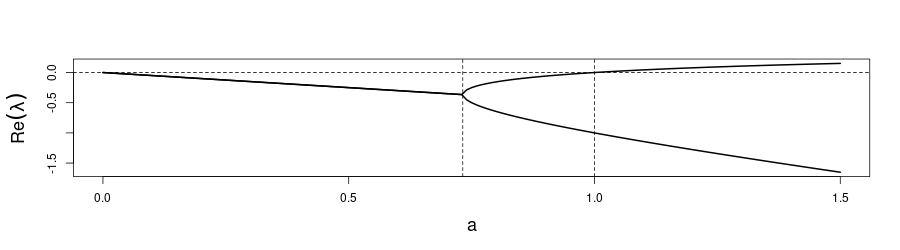
\includegraphics[width=.8\textwidth, trim=0 0 0 50, clip=]{LotkaVolterraDD-m0.5-eigenValueReal.png} \\
    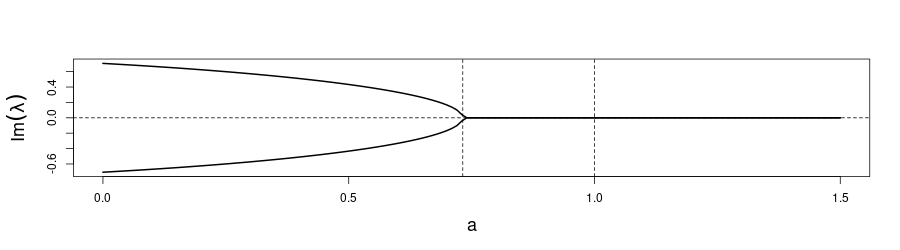
\includegraphics[width=.8\textwidth, trim=0 0 0 50, clip=]{LotkaVolterraDD-m0.5-eigenValueImaginary.png} 
  \end{array}
  $$
  La bifurcation se produit en $a = a_1$ et l'une des valeurs propres devient positive pour $a = a_2 = 1$.
  }
\end{enumerate}

\bigskip
\paragraph{Trajectoires.}
Les trajectoires ($i$), ($ii$) et ($iii$) suivantes ont été obtenues par intégration numérique avec $m = 1/2$ et partant de l'état initial $(x_0 = 3/2,\;  y_0 = 1)$ pour trois valeurs de $a$ différentes.
$$
\begin{array}{ccc}
  (i) & (ii) & (iii) \\
  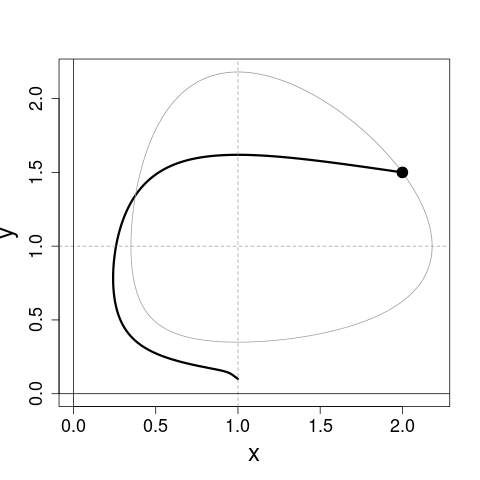
\includegraphics[width=.32\textwidth, trim=0 0 0 50, clip=]{LotkaVolterraDD-m0.5-a0.9.png} &
  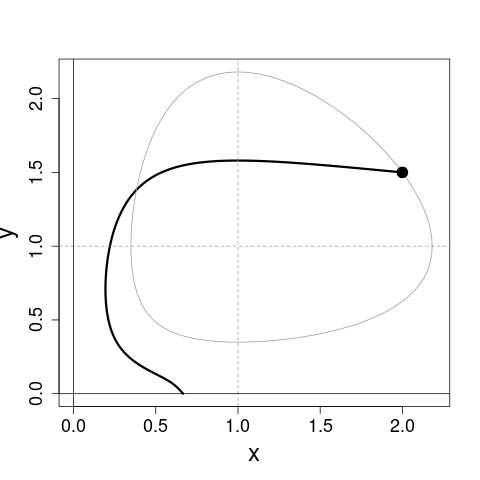
\includegraphics[width=.32\textwidth, trim=0 0 0 50, clip=]{LotkaVolterraDD-m0.5-a1.5.png} &
  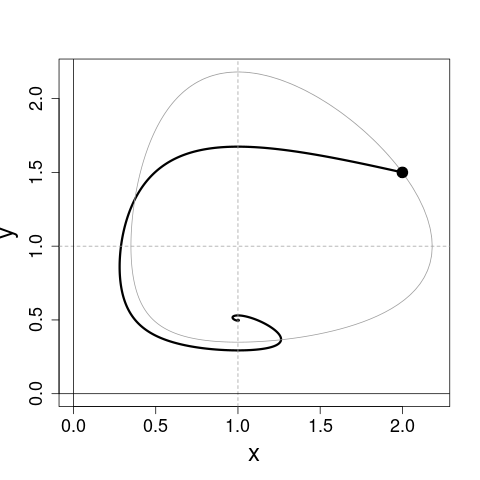
\includegraphics[width=.32\textwidth, trim=0 0 0 50, clip=]{LotkaVolterraDD-m0.5-a0.5.png}
\end{array}
$$
La courbe grise indique la trajectoire du modèle de Lotka-Volterra sans densité-dépendance ($m = 1/2$, $a = 0$). Les repères grisés indiquent l'état stationnaire de ce même modèle.

\begin{enumerate}
  \setcounter{enumi}{10}
  \item Associer chacune des trajectoires ($i$), ($ii$) et ($iii$) à l'une des trois valeurs de $a$ : $a = 1/2$, $a = 9/10$ ou $a = 3/2$.
  \solution{On a dans ce cas $a_1 = \sqrt{3} - 1 \simeq 0.73$ et $a_2 = 1$.
  \begin{description}
    \item[$a = 1/2 < a_1$ :] le système possède un équilibre stable en ($x^* = 1, y^* = 1/2$) et les valeurs propres de $J^*$ possèdent une partie imaginaire non nulle qui induit un enroulement autour de l'équilibre : on reconnaît la trajectoire ($iii$).
    \item[$a_1 < a = 9/10 < a_2$ :] le système possède un équilibre stable en ($x^* = 1, y^* = 1/10$) mais les valeurs propres de $J^*$ sont réelles et négatives : le système tend vers l'équilibre sans enroulement : on reconnaît la trajectoire ($i$).
    \item[$a = 3/2 > a_1$ :] le système possède un équilibre instable en ($x^* = 1, y^* = -1/2$) que le système n'atteint jamais, du fait de l'extinction des prédateurs ($y(t) \to 0$) : on reconnaît la trajectoire ($ii$).
  \end{description}
  }
  \item Donner la limite de $x(t)$ quand $t$ tend vers l'infini dans le cas ($ii$).
  \solution{
  Dans ce cas, $y(t)$ tend vers 0 quand $t \to\infty$, le système \eqref{eq:LVDD-Jstar} devient donc simplement $\dot x = F(x)$ avec $F(x) = x (1 - ax)$. Ce système adment deux point stationnaire en $x_1 = 0$ et $x_2 = 1/a$ et seul le second est stable (car $F'(x_1) > 0$ et $F'(x_2) < 0$). \\
  Après extinction des prédateurs, la population des proies tend donc vers $x_2 = 1/a = 2/3$ : elle n'explose donc pas, contrairement au modèle de Lotka-Volterra classique.
  }
\end{enumerate}
